%--- Implementation
\begin{figure}[H]
    \centering
    \caption{Plan Cuadrante and Changes in Police Resources}
    \label{fig:resources}
    \label{fig:figure_resources}
    \begin{tabular}{cc}
        \begin{minipage}[t]{0.48\textwidth}
            \centering
            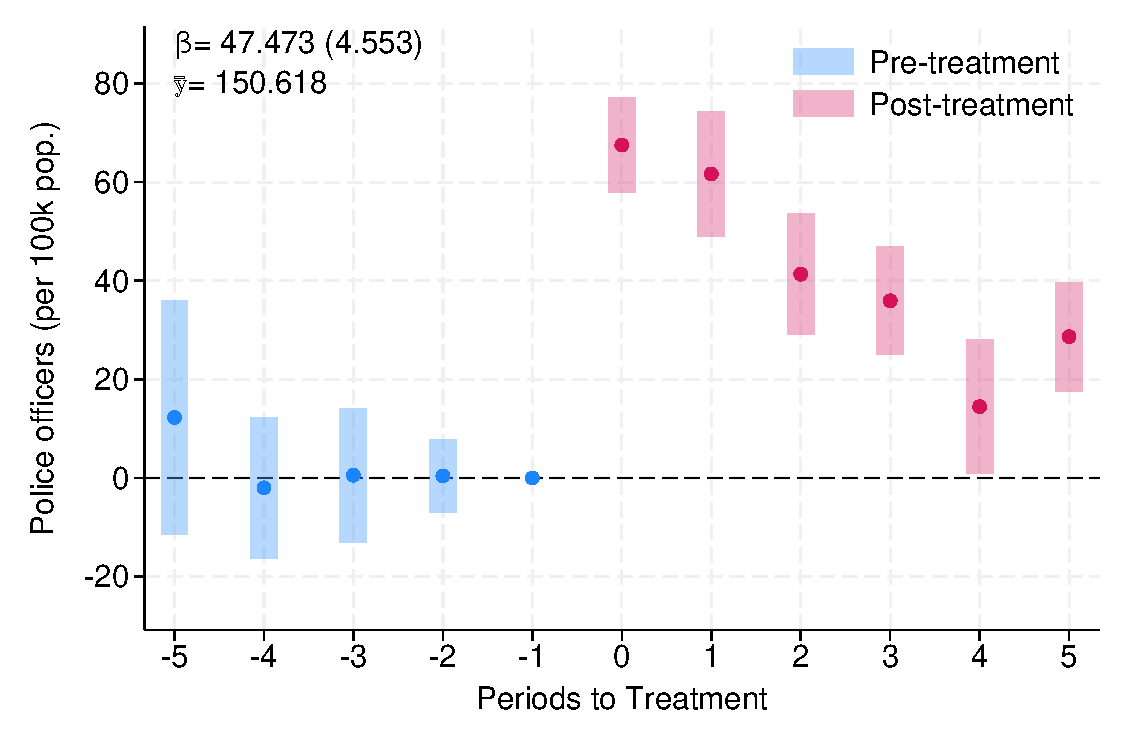
\includegraphics[width=\linewidth]{../manuscript/Graphs/fig4_officers.pdf}

            \small (a) Effect on the number of police officers
        \end{minipage}
        &
        \begin{minipage}[t]{0.48\textwidth}
            \centering
            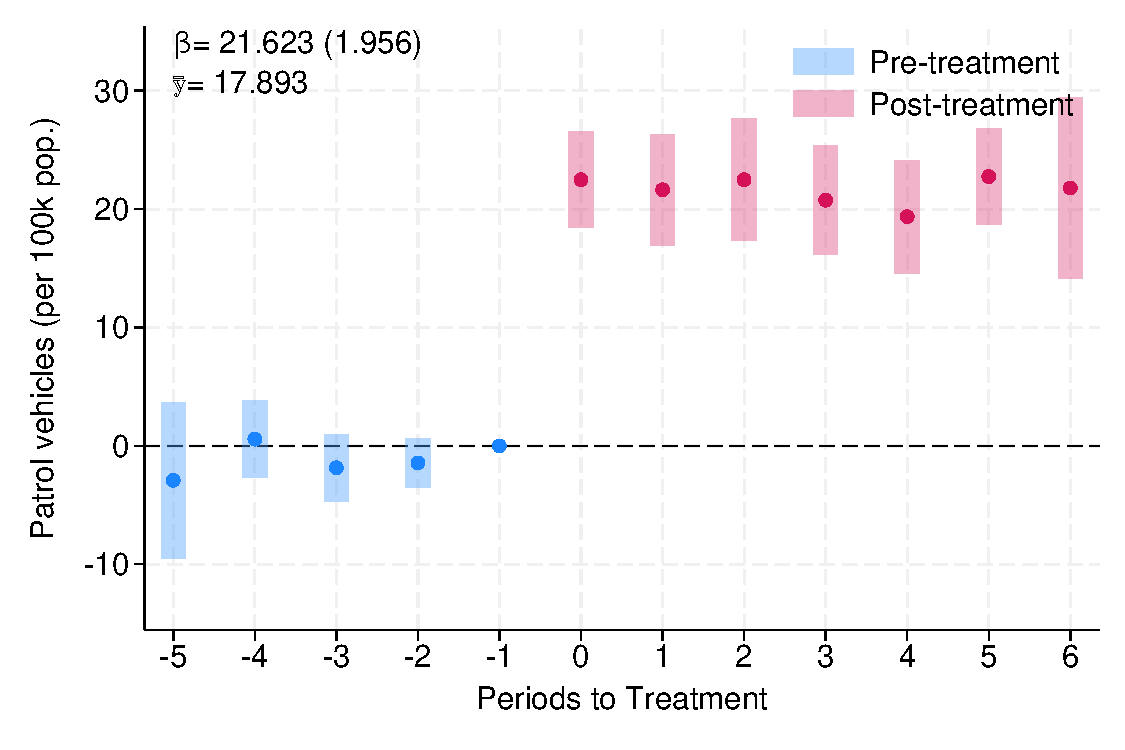
\includegraphics[width=\linewidth]{../manuscript/Graphs/fig4_patrols.pdf}

            \small (b) Effect on the number of patrol vehicles
        \end{minipage}
        \\[4pt]
        \begin{minipage}[t]{0.48\textwidth}
            \centering
            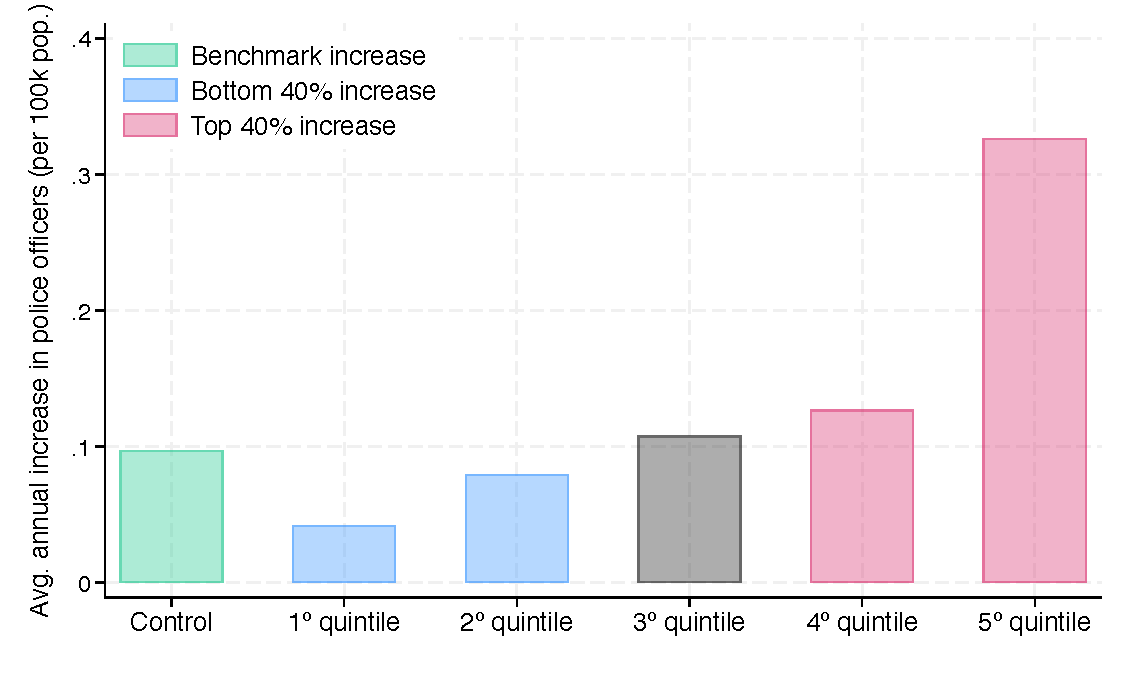
\includegraphics[width=\linewidth]{../manuscript/Graphs/increase_enusc_off_quintiles.pdf}

            \small (c) Distribution of $\Delta$ in police officers
        \end{minipage}
        &
        \begin{minipage}[t]{0.48\textwidth}
            \centering
            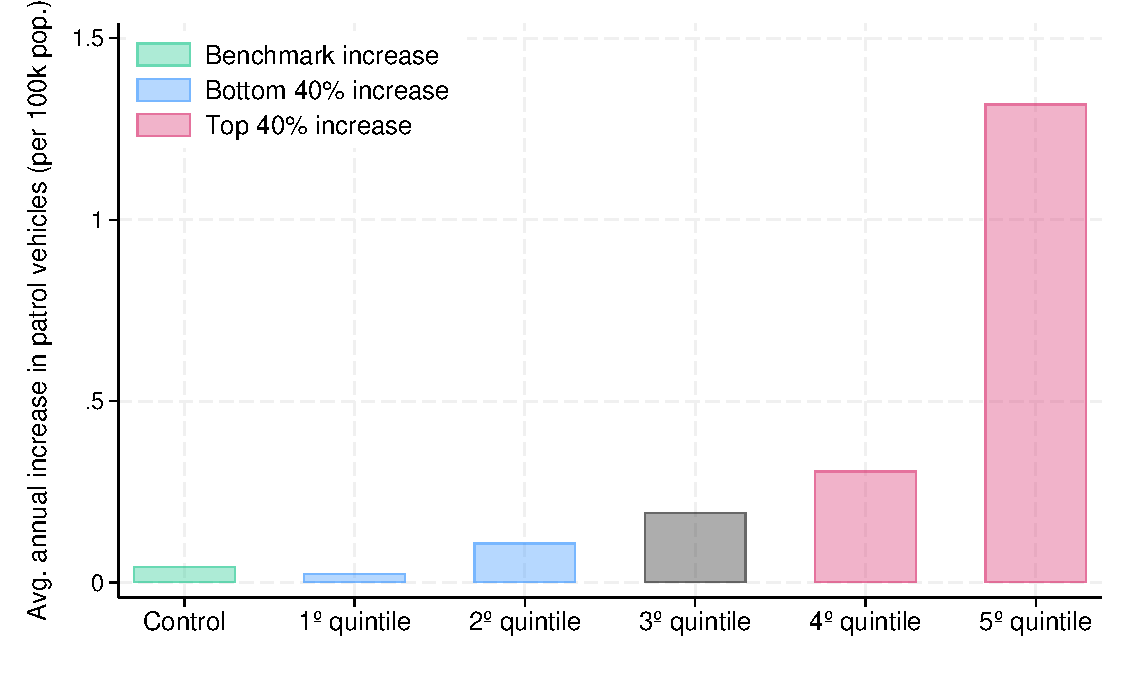
\includegraphics[width=\linewidth]{../manuscript/Graphs/increase_enusc_pv_quintiles.pdf}

            \small (d) Distribution of $\Delta$ in patrol vehicles
        \end{minipage}
        \\[4pt]
        \begin{minipage}[t]{0.48\textwidth}
            \centering
            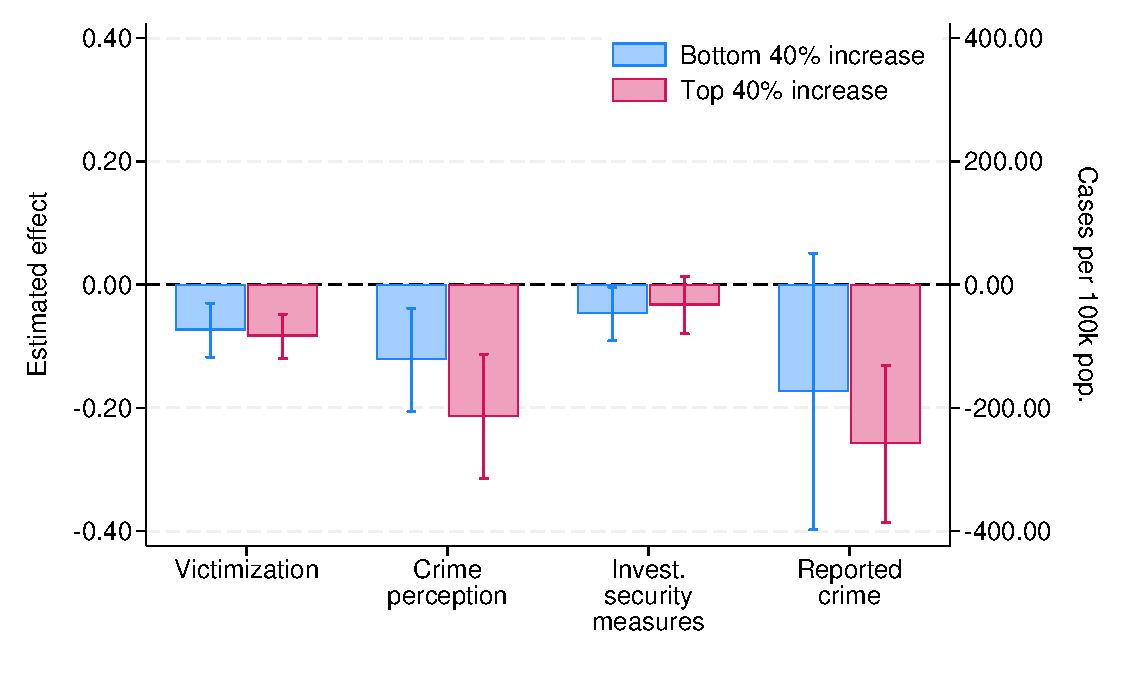
\includegraphics[width=\linewidth]{../manuscript/Graphs/heterogeneity_off.pdf}

            \small (e) Effects by the intensity of $\Delta$ in police officers
        \end{minipage}
        &
        \begin{minipage}[t]{0.48\textwidth}
            \centering
            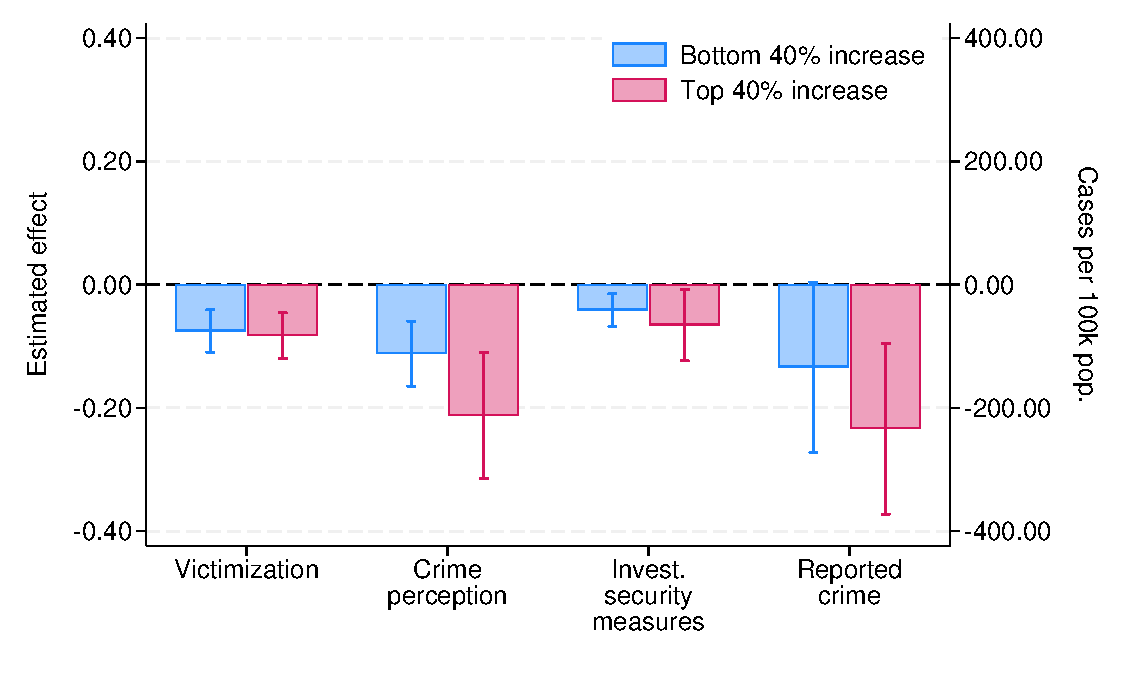
\includegraphics[width=\linewidth]{../manuscript/Graphs/heterogeneity_pv.pdf}

            \small (f) Effects by the intensity of $\Delta$ in patrol vehicles
        \end{minipage}
    \end{tabular}
    \vspace{4pt}
    \begin{minipage}{0.99\textwidth}
    \footnotesize Notes: Panels (a) and (b) show the effect of \emph{Plan Cuadrante} on police officers and patrol vehicles per 100,000 inhabitants. Panels (c) and (d) show the distribution of annual changes in officers and patrol vehicles across municipalities. Panels (e) and (f) report effects by the intensity of resource changes, comparing municipalities in the bottom 40\% and top 40\% of the distribution. The estimation follows \citet{Callaway}. The graphs display estimated coefficients and 95\% confidence intervals. Standard errors are clustered at the municipality level using wild bootstrapping.
    \end{minipage}
\end{figure}